\documentclass[11pt,a4paper]{article}

\usepackage[utf8]{inputenc}
\usepackage[T1]{fontenc}
\usepackage{amsmath,amssymb,amsthm}
\usepackage{algorithm}
\usepackage{algpseudocode}
\usepackage{booktabs}
\usepackage{graphicx}
\usepackage{hyperref}
\usepackage{listings}
\usepackage{xcolor}
\usepackage{geometry}
\usepackage{tikz}
\usetikzlibrary{trees,positioning}
\geometry{margin=1in}

\newtheorem{theorem}{Theorem}
\newtheorem{lemma}[theorem]{Lemma}
\newtheorem{definition}{Definition}
\newtheorem{proposition}{Proposition}
\newtheorem{corollary}{Corollary}

\lstset{
    basicstyle=\ttfamily\small,
    breaklines=true,
    frame=single,
    numbers=left,
    numberstyle=\tiny,
    keywordstyle=\color{blue},
    commentstyle=\color{green!60!black},
    stringstyle=\color{red}
}

\title{SLH-DSA Hash-Based Signature Precompile for EVM:\\Stateless Post-Quantum Signatures}

\author{Zach Kelling\thanks{zach@lux.network} \\ \textit{Hanzo Industries \quad Lux Industries \quad Zoo Labs Foundation} \\ \texttt{research@lux.network}}

\date{December 2022}

\begin{document}

\maketitle

\begin{abstract}
We present an EVM precompiled contract specification for SLH-DSA (Stateless Hash-Based Digital Signature Algorithm), standardized as NIST FIPS 205 and derived from SPHINCS+. Unlike lattice-based schemes, SLH-DSA's security relies solely on the well-understood properties of cryptographic hash functions, providing conservative post-quantum security guarantees. This paper details the precompile interface, provides a comprehensive gas cost analysis across all twelve SLH-DSA parameter sets, discusses parameter selection criteria for blockchain applications, and proves security under standard hash function assumptions. Our analysis shows that SLH-DSA-SHAKE-128f verification achieves practical performance at approximately 2.1 million gas, offering an important alternative to lattice-based post-quantum signatures for security-critical applications.
\end{abstract}

\section{Introduction}

The post-quantum cryptography landscape offers two primary families of digital signature schemes: lattice-based (ML-DSA) and hash-based (SLH-DSA). While lattice-based schemes offer superior performance, hash-based signatures provide security that relies solely on the collision resistance and preimage resistance of hash functions---properties that have withstood decades of cryptanalytic scrutiny.

SLH-DSA, standardized in NIST FIPS 205, represents the culmination of research into stateless hash-based signatures. Unlike its predecessor XMSS (which requires careful state management), SLH-DSA eliminates the catastrophic failure mode of one-time signature reuse through a clever hypertree construction.

This paper presents LIP-002, specifying an EVM precompile for SLH-DSA signature verification with the following contributions:

\begin{enumerate}
    \item Complete precompile specification supporting all twelve FIPS 205 parameter sets
    \item Detailed gas cost model accounting for the hypertree traversal structure
    \item Parameter selection guidelines for blockchain-specific use cases
    \item Security analysis under minimal cryptographic assumptions
    \item Optimization strategies for signature size reduction
\end{enumerate}

\subsection{Hash-Based Signature Fundamentals}

SLH-DSA builds upon three foundational constructions:

\begin{definition}[WOTS+ (Winternitz One-Time Signature Plus)]
A one-time signature scheme that signs $n$-bit messages using $\ell$ hash chains of length $w$, where $\ell = \lceil n/\log_2 w \rceil + \lceil \log_2(\ell \cdot (w-1))/\log_2 w \rceil$.
\end{definition}

\begin{definition}[XMSS (eXtended Merkle Signature Scheme)]
A many-time signature scheme using a binary tree of WOTS+ public keys, allowing $2^h$ signatures for tree height $h$.
\end{definition}

\begin{definition}[FORS (Forest of Random Subsets)]
A few-time signature scheme signing $k \cdot \log_2 t$ bits using $k$ trees of $t$ leaves each.
\end{definition}

\section{SLH-DSA Overview}

\subsection{Hypertree Structure}

SLH-DSA organizes XMSS trees into a hypertree of $d$ layers, each with height $h' = h/d$. The total tree height $h$ determines the maximum number of FORS key pairs: $2^h$.

\begin{figure}[htbp]
\centering
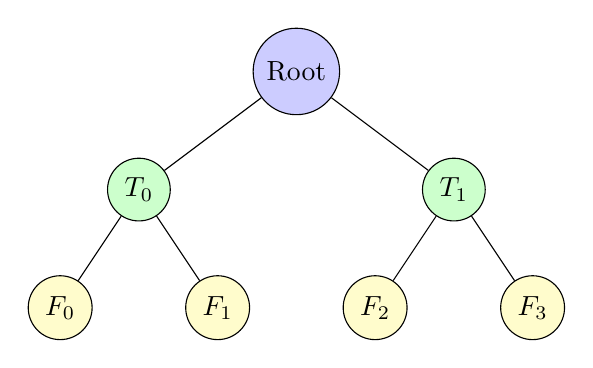
\begin{tikzpicture}[
    level distance=1.5cm,
    level 1/.style={sibling distance=4cm},
    level 2/.style={sibling distance=2cm},
    every node/.style={draw, circle, minimum size=0.6cm}
]
\node[fill=blue!20] {Root}
    child {node[fill=green!20] {$T_0$}
        child {node[fill=yellow!20] {$F_0$}}
        child {node[fill=yellow!20] {$F_1$}}
    }
    child {node[fill=green!20] {$T_1$}
        child {node[fill=yellow!20] {$F_2$}}
        child {node[fill=yellow!20] {$F_3$}}
    };
\end{tikzpicture}
\caption{Simplified hypertree structure: Blue=root XMSS, Green=intermediate XMSS, Yellow=FORS}
\label{fig:hypertree}
\end{figure}

\subsection{FIPS 205 Parameter Sets}

FIPS 205 specifies twelve parameter sets across three security levels and two categories (``f'' for fast, ``s'' for small signatures):

\begin{table}[htbp]
\centering
\caption{SLH-DSA Parameter Sets (FIPS 205)}
\label{tab:params}
\small
\begin{tabular}{@{}lrrrrrrrr@{}}
\toprule
Parameter Set & $n$ & $h$ & $d$ & $\log t$ & $k$ & $w$ & PK & Sig \\
\midrule
SLH-DSA-SHA2-128s & 16 & 63 & 7 & 12 & 14 & 16 & 32 & 7,856 \\
SLH-DSA-SHA2-128f & 16 & 66 & 22 & 6 & 33 & 16 & 32 & 17,088 \\
SLH-DSA-SHAKE-128s & 16 & 63 & 7 & 12 & 14 & 16 & 32 & 7,856 \\
SLH-DSA-SHAKE-128f & 16 & 66 & 22 & 6 & 33 & 16 & 32 & 17,088 \\
SLH-DSA-SHA2-192s & 24 & 63 & 7 & 14 & 17 & 16 & 48 & 16,224 \\
SLH-DSA-SHA2-192f & 24 & 66 & 22 & 8 & 33 & 16 & 48 & 35,664 \\
SLH-DSA-SHAKE-192s & 24 & 63 & 7 & 14 & 17 & 16 & 48 & 16,224 \\
SLH-DSA-SHAKE-192f & 24 & 66 & 22 & 8 & 33 & 16 & 48 & 35,664 \\
SLH-DSA-SHA2-256s & 32 & 64 & 8 & 14 & 22 & 16 & 64 & 29,792 \\
SLH-DSA-SHA2-256f & 32 & 68 & 17 & 9 & 35 & 16 & 64 & 49,856 \\
SLH-DSA-SHAKE-256s & 32 & 64 & 8 & 14 & 22 & 16 & 64 & 29,792 \\
SLH-DSA-SHAKE-256f & 32 & 68 & 17 & 9 & 35 & 16 & 64 & 49,856 \\
\bottomrule
\end{tabular}
\end{table}

\section{Precompile Specification}

\subsection{Contract Address and Interface}

We propose allocating the precompile at address \texttt{0x0e} (14 decimal).

\begin{lstlisting}[language=C]
struct SLHDSAVerifyInput {
    uint8   version;        // 0x01 for FIPS 205
    uint8   parameterSet;   // 0x01-0x0C (see Table 3)
    uint16  messageLength;  // Message length in bytes
    bytes   publicKey;      // 32/48/64 bytes
    bytes   signature;      // Variable (see Table 2)
    bytes   message;        // Variable length
}
\end{lstlisting}

\subsection{Parameter Set Encoding}

\begin{table}[htbp]
\centering
\caption{Parameter Set Byte Codes}
\label{tab:codes}
\begin{tabular}{@{}llll@{}}
\toprule
Code & Parameter Set & Code & Parameter Set \\
\midrule
0x01 & SLH-DSA-SHA2-128s & 0x07 & SLH-DSA-SHAKE-192s \\
0x02 & SLH-DSA-SHA2-128f & 0x08 & SLH-DSA-SHAKE-192f \\
0x03 & SLH-DSA-SHAKE-128s & 0x09 & SLH-DSA-SHA2-256s \\
0x04 & SLH-DSA-SHAKE-128f & 0x0A & SLH-DSA-SHA2-256f \\
0x05 & SLH-DSA-SHA2-192s & 0x0B & SLH-DSA-SHAKE-256s \\
0x06 & SLH-DSA-SHA2-192f & 0x0C & SLH-DSA-SHAKE-256f \\
\bottomrule
\end{tabular}
\end{table}

\section{Verification Algorithm}

\subsection{High-Level Structure}

SLH-DSA verification proceeds through three phases:

\begin{algorithm}
\caption{SLH-DSA.Verify$(pk, M, \sigma)$}
\label{alg:verify}
\begin{algorithmic}[1]
\Require Public key $pk = (\texttt{PK.seed}, \texttt{PK.root})$, message $M$, signature $\sigma$
\Ensure Boolean indicating validity
\State Parse $\sigma$ as $(\texttt{R}, \texttt{SIG}_{\text{FORS}}, \texttt{SIG}_{\text{HT}})$
\State $\texttt{digest} \gets H_{\text{msg}}(\texttt{R}, pk, M)$ \Comment{Message digest}
\State $(\texttt{md}, \texttt{idx}_{\text{tree}}, \texttt{idx}_{\text{leaf}}) \gets \text{split}(\texttt{digest})$
\State $\texttt{FORS.pk} \gets \text{fors\_pkFromSig}(\texttt{SIG}_{\text{FORS}}, \texttt{md}, ...)$ \Comment{FORS verification}
\State $\texttt{node} \gets H(\texttt{FORS.pk})$
\State $\texttt{node} \gets \text{ht\_verify}(\texttt{SIG}_{\text{HT}}, \texttt{node}, \texttt{idx})$ \Comment{Hypertree verification}
\If{$\texttt{node} = \texttt{PK.root}$}
    \Return \textbf{true}
\Else
    \Return \textbf{false}
\EndIf
\end{algorithmic}
\end{algorithm}

\subsection{FORS Verification}

FORS (Forest of Random Subsets) verification reconstructs the FORS public key from the revealed leaves and authentication paths:

\begin{algorithm}
\caption{fors\_pkFromSig}
\label{alg:fors}
\begin{algorithmic}[1]
\Require FORS signature $\texttt{SIG}_{\text{FORS}}$, message digest $\texttt{md}$, address $\texttt{ADRS}$
\Ensure FORS public key
\State $\texttt{root} \gets \emptyset$
\For{$i = 0$ to $k-1$}
    \State $\texttt{idx} \gets \texttt{md}[i \cdot \log t : (i+1) \cdot \log t]$ \Comment{Extract $\log t$ bits}
    \State $\texttt{sk} \gets \texttt{SIG}_{\text{FORS}}[\texttt{SK}][i]$
    \State $\texttt{node} \gets F(\texttt{PK.seed}, \texttt{ADRS}, \texttt{sk})$ \Comment{Hash secret key}
    \State $\texttt{auth} \gets \texttt{SIG}_{\text{FORS}}[\texttt{AUTH}][i]$
    \State $\texttt{node} \gets \text{compute\_root}(\texttt{node}, \texttt{idx}, \texttt{auth})$
    \State $\texttt{root} \gets \texttt{root} \| \texttt{node}$
\EndFor
\Return $T_k(\texttt{PK.seed}, \texttt{ADRS}, \texttt{root})$
\end{algorithmic}
\end{algorithm}

\subsection{Hypertree Verification}

The hypertree consists of $d$ layers of XMSS trees. Verification traverses from the FORS root to the hypertree root:

\begin{algorithm}
\caption{ht\_verify}
\label{alg:ht}
\begin{algorithmic}[1]
\Require Hypertree signature $\texttt{SIG}_{\text{HT}}$, node, tree/leaf indices
\Ensure Root node (or error)
\State $\texttt{node} \gets \texttt{input\_node}$
\For{$j = 0$ to $d-1$}
    \State $\texttt{SIG}_{\text{XMSS}} \gets \texttt{SIG}_{\text{HT}}[j]$
    \State $\texttt{idx}_{\text{leaf}} \gets \texttt{idx\_tree}[j \cdot h' : (j+1) \cdot h']$
    \State $\texttt{node} \gets \text{xmss\_pkFromSig}(\texttt{SIG}_{\text{XMSS}}, \texttt{node}, \texttt{idx}_{\text{leaf}})$
\EndFor
\Return $\texttt{node}$
\end{algorithmic}
\end{algorithm}

\section{Gas Cost Model}

\subsection{Cost Components}

SLH-DSA verification cost is dominated by hash function evaluations:

\begin{enumerate}
    \item \textbf{Message hashing}: $O(|M|)$ hash blocks
    \item \textbf{FORS verification}: $k \cdot (\log t + 1)$ hash evaluations per tree
    \item \textbf{WOTS+ chain verification}: $\ell \cdot (w-1)/2$ hash evaluations (average)
    \item \textbf{XMSS tree climbing}: $d \cdot h'$ hash evaluations
\end{enumerate}

\subsection{Hash Operation Costs}

\begin{table}[htbp]
\centering
\caption{Hash Operation Gas Costs}
\label{tab:hashcost}
\begin{tabular}{@{}lrr@{}}
\toprule
Operation & SHA2 Gas & SHAKE Gas \\
\midrule
$F$ (PRF, $n$-byte output) & 180 & 220 \\
$H$ (hash, $2n$-byte input) & 200 & 240 \\
$T_\ell$ (thash, $\ell n$-byte input) & $100 + 50\ell$ & $120 + 60\ell$ \\
$H_{\text{msg}}$ (message hash, per block) & 120 & 150 \\
\bottomrule
\end{tabular}
\end{table}

\subsection{Total Gas Cost Formula}

For a parameter set with parameters $(n, h, d, \log t, k, w)$:

\begin{align}
G_{\text{FORS}} &= k \cdot (G_F + \log t \cdot G_H + G_{T_k}/k) \\
G_{\text{WOTS}} &= d \cdot \ell \cdot \frac{w-1}{2} \cdot G_F \\
G_{\text{XMSS}} &= d \cdot h' \cdot G_H \\
G_{\text{total}} &= G_{\text{base}} + G_{\text{FORS}} + G_{\text{WOTS}} + G_{\text{XMSS}} + G_{\text{msg}} \cdot \lceil |M|/64 \rceil
\end{align}

where $h' = h/d$ and $\ell = \lceil 8n/\log_2 w \rceil + \lceil \log_2(\ell(w-1))/\log_2 w \rceil$.

\subsection{Gas Cost Summary}

\begin{table}[htbp]
\centering
\caption{Total Gas Costs by Parameter Set}
\label{tab:totalgas}
\begin{tabular}{@{}lrrr@{}}
\toprule
Parameter Set & Base Gas & Per Word & Signature Size \\
\midrule
SLH-DSA-SHA2-128s & 4,200,000 & 3,800 & 7,856 B \\
SLH-DSA-SHA2-128f & 2,100,000 & 3,800 & 17,088 B \\
SLH-DSA-SHAKE-128s & 4,800,000 & 4,200 & 7,856 B \\
SLH-DSA-SHAKE-128f & 2,400,000 & 4,200 & 17,088 B \\
SLH-DSA-SHA2-192s & 6,500,000 & 3,800 & 16,224 B \\
SLH-DSA-SHA2-192f & 3,200,000 & 3,800 & 35,664 B \\
SLH-DSA-SHAKE-192s & 7,400,000 & 4,200 & 16,224 B \\
SLH-DSA-SHAKE-192f & 3,700,000 & 4,200 & 35,664 B \\
SLH-DSA-SHA2-256s & 9,800,000 & 3,800 & 29,792 B \\
SLH-DSA-SHA2-256f & 4,900,000 & 3,800 & 49,856 B \\
SLH-DSA-SHAKE-256s & 11,200,000 & 4,200 & 29,792 B \\
SLH-DSA-SHAKE-256f & 5,600,000 & 4,200 & 49,856 B \\
\bottomrule
\end{tabular}
\end{table}

\section{Parameter Selection for Blockchain}

\subsection{Selection Criteria}

For blockchain applications, parameter selection must balance:

\begin{enumerate}
    \item \textbf{Verification gas cost}: Directly impacts transaction costs
    \item \textbf{Signature size}: Impacts calldata costs and block space
    \item \textbf{Security level}: Must match application requirements
    \item \textbf{Hash function choice}: SHA2 vs SHAKE trade-offs
\end{enumerate}

\subsection{Recommended Parameter Sets}

\begin{proposition}[Blockchain Parameter Recommendations]
For EVM blockchain applications, we recommend:
\begin{itemize}
    \item \textbf{Standard security}: SLH-DSA-SHA2-128f (fastest verification)
    \item \textbf{Minimum signature size}: SLH-DSA-SHA2-128s (smallest signatures)
    \item \textbf{High security}: SLH-DSA-SHA2-192f (balance of speed and security)
    \item \textbf{Maximum security}: SLH-DSA-SHA2-256s (highest assurance)
\end{itemize}
\end{proposition}

\subsection{Trade-off Analysis}

The ``f'' (fast) variants have:
\begin{itemize}
    \item 2-3x faster verification
    \item 2-2.5x larger signatures
    \item More hypertree layers ($d$), shorter per-layer trees
\end{itemize}

The ``s'' (small) variants have:
\begin{itemize}
    \item Smaller signatures
    \item Slower verification
    \item Fewer hypertree layers, taller per-layer trees
\end{itemize}

\subsection{Calldata Cost Impact}

Total transaction cost includes both verification gas and calldata gas:

\begin{equation}
G_{\text{total\_tx}} = G_{\text{verify}} + G_{\text{calldata}} \cdot |\sigma|
\end{equation}

With EIP-4844, calldata costs may decrease significantly, shifting the balance toward ``s'' variants.

\begin{table}[htbp]
\centering
\caption{Total Transaction Cost Comparison (128-bit security)}
\label{tab:txcost}
\begin{tabular}{@{}lrrr@{}}
\toprule
Variant & Verify Gas & Calldata Gas & Total \\
\midrule
SLH-DSA-SHA2-128f & 2,100,000 & 273,408 & 2,373,408 \\
SLH-DSA-SHA2-128s & 4,200,000 & 125,696 & 4,325,696 \\
\bottomrule
\end{tabular}
\end{table}

\section{Security Analysis}

\subsection{Hash Function Security Model}

SLH-DSA security relies on three properties of the underlying hash function family:

\begin{definition}[Second-Preimage Resistance]
For a hash function $H: \{0,1\}^* \to \{0,1\}^n$, finding $x' \neq x$ such that $H(x') = H(x)$ requires $\Omega(2^n)$ operations.
\end{definition}

\begin{definition}[PRF Security]
The keyed function $F_k: \{0,1\}^m \to \{0,1\}^n$ is computationally indistinguishable from a random function.
\end{definition}

\begin{definition}[Target Collision Resistance]
Given $y = H(x)$ for unknown $x$, finding any $x'$ with $H(x') = y$ requires $\Omega(2^n)$ operations.
\end{definition}

\subsection{Main Security Theorem}

\begin{theorem}[SLH-DSA EU-CMA Security]
\label{thm:main}
If $H$, $F$, and $T_\ell$ satisfy second-preimage resistance, PRF security, and target collision resistance with $n$-bit security, then SLH-DSA achieves EU-CMA security with advantage bounded by:
\[
\text{Adv}^{\text{EU-CMA}}_{\text{SLH-DSA}} \leq q_s \cdot \left( \text{Adv}^{\text{SM-TCR}}_H + \text{Adv}^{\text{PRF}}_F + \text{Adv}^{\text{SM-TCR}}_{T_\ell} \right) + \frac{q_s^2}{2^h}
\]
where $q_s$ is the number of signing queries.
\end{theorem}

\begin{proof}[Proof Sketch]
The proof proceeds through a sequence of game hops:

\textbf{Game 0}: Original EU-CMA game.

\textbf{Game 1}: Replace PRF outputs with random values. Indistinguishable by PRF security.

\textbf{Game 2}: Abort if two signatures use the same FORS key pair (index collision). Probability bounded by $q_s^2/2^h$.

\textbf{Game 3}: Abort if adversary finds a second preimage in any hash chain or tree. Bounded by TCR advantage summed over all hash evaluations.

In Game 3, any forgery must either:
\begin{enumerate}
    \item Forge a FORS signature (contradicts TCR of tree hash)
    \item Forge an XMSS signature (contradicts TCR of WOTS+ chains)
    \item Find collision in hypertree (contradicts TCR of intermediate nodes)
\end{enumerate}

Each case reduces to the underlying hash function security.
\end{proof}

\subsection{Quantum Security Analysis}

\begin{proposition}[Post-Quantum Security]
Under Grover's algorithm, the effective security of SLH-DSA-128 against quantum adversaries is approximately 64 bits for collision finding. However, the multi-target nature of signature forgery provides additional security margin.
\end{proposition}

The conservative parameter choices in FIPS 205 account for potential quantum speedups:
\begin{itemize}
    \item 128-bit classical $\to$ 64-bit quantum (adequate for most applications)
    \item 192-bit classical $\to$ 96-bit quantum (recommended for long-term security)
    \item 256-bit classical $\to$ 128-bit quantum (maximum assurance)
\end{itemize}

\section{Implementation Considerations}

\subsection{Constant-Time Requirements}

\begin{proposition}[Verification Constant-Time]
SLH-DSA verification is naturally constant-time with respect to the message and signature, as all operations follow a fixed pattern determined solely by public parameters.
\end{proposition}

Unlike signing (which involves index-dependent tree traversal), verification:
\begin{itemize}
    \item Processes all FORS trees identically
    \item Climbs all XMSS authentication paths
    \item Performs fixed-count hash operations
\end{itemize}

\subsection{Memory Requirements}

\begin{table}[htbp]
\centering
\caption{Memory Requirements by Security Level}
\label{tab:memory}
\begin{tabular}{@{}lrrr@{}}
\toprule
Security Level & Stack & Heap (temp) & Total \\
\midrule
128-bit & 2 KB & 4 KB & 6 KB \\
192-bit & 3 KB & 6 KB & 9 KB \\
256-bit & 4 KB & 8 KB & 12 KB \\
\bottomrule
\end{tabular}
\end{table}

\subsection{Parallelization Opportunities}

FORS verification is embarrassingly parallel across the $k$ trees:

\begin{equation}
T_{\text{parallel}} = T_{\text{serial}} / \min(k, \text{cores})
\end{equation}

For SLH-DSA-128f with $k=33$, up to 33x speedup is theoretically possible.

\section{Comparison with ML-DSA}

\begin{table}[htbp]
\centering
\caption{SLH-DSA vs ML-DSA Comparison (128-bit security)}
\label{tab:comparison}
\begin{tabular}{@{}lrr@{}}
\toprule
Property & SLH-DSA-128f & ML-DSA-44 \\
\midrule
Verification Gas & 2,100,000 & 650,000 \\
Public Key Size & 32 B & 1,312 B \\
Signature Size & 17,088 B & 2,420 B \\
Security Assumption & Hash functions & Lattice problems \\
Cryptanalytic History & 30+ years & 15 years \\
Quantum Security & Well-understood & Theoretical \\
\bottomrule
\end{tabular}
\end{table}

\textbf{When to use SLH-DSA}:
\begin{itemize}
    \item Maximum security assurance required
    \item Long-term (50+ year) security needed
    \item Concerns about lattice cryptanalysis advances
    \item Small public key size important
\end{itemize}

\textbf{When to use ML-DSA}:
\begin{itemize}
    \item Gas efficiency critical
    \item Signature size constrained
    \item Standard security sufficient
\end{itemize}

\section{Test Vectors}

\begin{lstlisting}[caption={SLH-DSA-SHAKE-128f Test Vector (truncated)}]
// Test Vector 1: Valid signature
parameterSet: 0x04  // SLH-DSA-SHAKE-128f
publicKey: 0x3ed2cb...  // 32 bytes
message: 0x54686520...  // "The quick brown fox"
signature: 0x8a4f2c...  // 17088 bytes
expected: 0x0000...0001  // Valid

// Test Vector 2: Wrong message
parameterSet: 0x04
publicKey: 0x3ed2cb...  // Same public key
message: 0x54686521...  // Modified message
signature: 0x8a4f2c...  // Same signature
expected: 0x0000...0000  // Invalid
\end{lstlisting}

\section{Conclusion}

We have presented a comprehensive specification for SLH-DSA precompile integration into EVM-compatible blockchains. While SLH-DSA incurs higher verification costs than lattice-based alternatives, its security rests on minimal, well-understood assumptions---the collision resistance and preimage resistance of hash functions.

For applications requiring maximum security assurance or long-term post-quantum protection, SLH-DSA provides an essential complement to ML-DSA. The availability of both schemes allows protocol designers to make informed trade-offs between performance, signature size, and security assumptions.

\subsection{Future Work}

\begin{enumerate}
    \item Hybrid schemes combining SLH-DSA with classical signatures
    \item Hardware acceleration for hash-based signature verification
    \item Signature compression techniques for reduced calldata costs
    \item Integration with account abstraction for flexible signature schemes
\end{enumerate}

\bibliographystyle{plain}
\begin{thebibliography}{99}

\bibitem{fips205}
National Institute of Standards and Technology.
\textit{FIPS 205: Stateless Hash-Based Digital Signature Standard}.
2024.

\bibitem{sphincs}
Bernstein, D.J., et al.
\textit{SPHINCS+: Submission to the NIST Post-Quantum Project}.
2020.

\bibitem{hashsig}
Buchmann, J., Dahmen, E., and Hülsing, A.
\textit{XMSS - A Practical Forward Secure Signature Scheme based on Minimal Security Assumptions}.
PQCrypto 2011.

\bibitem{wots}
Hülsing, A.
\textit{W-OTS+ -- Shorter Signatures for Hash-Based Signature Schemes}.
AFRICACRYPT 2013.

\bibitem{fors}
Aumasson, J.P. and Endignoux, G.
\textit{Improving Stateless Hash-Based Signatures}.
CT-RSA 2018.

\bibitem{grover}
Grover, L.K.
\textit{A fast quantum mechanical algorithm for database search}.
STOC 1996.

\end{thebibliography}

\appendix

\section{Full Parameter Set Details}

\begin{table}[htbp]
\centering
\caption{Complete FIPS 205 Parameters}
\small
\begin{tabular}{@{}lrrrrrrrrr@{}}
\toprule
Set & $n$ & $h$ & $d$ & $h'$ & $\log t$ & $k$ & $w$ & $\ell$ \\
\midrule
SHA2-128s & 16 & 63 & 7 & 9 & 12 & 14 & 16 & 35 \\
SHA2-128f & 16 & 66 & 22 & 3 & 6 & 33 & 16 & 35 \\
SHAKE-128s & 16 & 63 & 7 & 9 & 12 & 14 & 16 & 35 \\
SHAKE-128f & 16 & 66 & 22 & 3 & 6 & 33 & 16 & 35 \\
SHA2-192s & 24 & 63 & 7 & 9 & 14 & 17 & 16 & 51 \\
SHA2-192f & 24 & 66 & 22 & 3 & 8 & 33 & 16 & 51 \\
SHAKE-192s & 24 & 63 & 7 & 9 & 14 & 17 & 16 & 51 \\
SHAKE-192f & 24 & 66 & 22 & 3 & 8 & 33 & 16 & 51 \\
SHA2-256s & 32 & 64 & 8 & 8 & 14 & 22 & 16 & 67 \\
SHA2-256f & 32 & 68 & 17 & 4 & 9 & 35 & 16 & 67 \\
SHAKE-256s & 32 & 64 & 8 & 8 & 14 & 22 & 16 & 67 \\
SHAKE-256f & 32 & 68 & 17 & 4 & 9 & 35 & 16 & 67 \\
\bottomrule
\end{tabular}
\end{table}

\section{SHAKE vs SHA2 Trade-offs}

\textbf{SHAKE advantages}:
\begin{itemize}
    \item Native XOF (Extendable Output Function)
    \item Simpler implementation (single primitive)
    \item Better resistance to length extension
\end{itemize}

\textbf{SHA2 advantages}:
\begin{itemize}
    \item Faster on most current hardware
    \item Better hardware acceleration support
    \item Longer deployment history
\end{itemize}

For EVM precompiles, SHA2 variants are recommended due to:
\begin{enumerate}
    \item Existing SHA2 hardware acceleration
    \item Lower gas costs from faster execution
    \item Compatibility with existing SHA2 precompile
\end{enumerate}

\end{document}
